% 
% Annual Cognitive Science Conference
% Sample LaTeX Paper -- Proceedings Format
% 

% Original : Ashwin Ram (ashwin@cc.gatech.edu)       04/01/1994
% Modified : Johanna Moore (jmoore@cs.pitt.edu)      03/17/1995
% Modified : David Noelle (noelle@ucsd.edu)          03/15/1996
% Modified : Pat Langley (langley@cs.stanford.edu)   01/26/1997
% Latex2e corrections by Ramin Charles Nakisa        01/28/1997 
% Modified : Tina Eliassi-Rad (eliassi@cs.wisc.edu)  01/31/1998
% Modified : Trisha Yannuzzi (trisha@ircs.upenn.edu) 12/28/1999 (in process)
% Modified : Mary Ellen Foster (M.E.Foster@ed.ac.uk) 12/11/2000
% Modified : Ken Forbus                              01/23/2004
% Modified : Eli M. Silk (esilk@pitt.edu)            05/24/2005
% Modified : Niels Taatgen (taatgen@cmu.edu)         10/24/2006
% Modified : David Noelle (dnoelle@ucmerced.edu)     11/19/2014

%% Change "letterpaper" in the following line to "a4paper" if you must.

\documentclass[10pt,letterpaper]{article}

\usepackage{cogsci}
\usepackage{commath}
\usepackage{graphicx}
\usepackage{pslatex}
\usepackage{apacite}


\title{TODO title}
 
\author{{\large \bf Jan Gosmann (jgosmann@uwaterloo.ca)} \\
  %Department of Psychology, 1202 W. Johnson Street \\
  %Madison, WI 53706 USA
  \AND{\large \bf Aaron Voelker (TODO)} \\
  \AND{\large \bf Chris Eliasmith (TODO)}
  %Department of Educational Psychology, 1025 W. Johnson Street \\
  %Madison, WI 53706 USA}
  }


\begin{document}

\maketitle


\begin{abstract}
The abstract should be one paragraph, indented 1/8~inch on both sides,
in 9~point font with single spacing. The heading ``{\bf Abstract}''
should be 10~point, bold, centered, with one line of space below
it. This one-paragraph abstract section is required only for standard
six page proceedings papers. Following the abstract should be a blank
line, followed by the header ``{\bf Keywords:}'' and a list of
descriptive keywords separated by semicolons, all in 9~point font, as
shown below.

\textbf{Keywords:} 
add your choice of indexing terms or keywords; kindly use a
semicolon; between each term
\end{abstract}


\section{Introduction}
Winner-take-all (WTA) mechanisms are often employed in cognitive 
models~\cite<e.g.,>{oreilly1998}.  A WTA mechanism receives a $d$-dimensional 
input of utility values for $d$ different choices. The output is supposed to be 
larger than zero for the dimension with highest utility and zero for all other 
inputs.

A large body of literature exists examining the optimality of WTA mechanisms and 
their consistency with neurobiological and psychological 
data~\cite<e.g.,>{bogacz2006,gold2007,smith2004}.  Here, however, we will 
investigate the suitability of two different WTA mechanisms in the context of 
large-scale cognitive modelling with spiking neurons on a set of benchmarks that 
are more normative in nature.  The first mechanism is an implementation of the 
classic leaky, competing accumulator model by~\citeA{usher2001}.  It has been 
widely used, for example in versions of the Temporal Context 
Model~\cite{sederberg2008}, and some of our models~\cite<e.g.,>{kajic2017}. We 
will compare this to an independent accumulator model with a second thresholding 
layer with recurrent connections to the first layer.  In both cases we are 
especially interested in situations with more than two ($d > 2$) choices.

For the implementation of these models we use the Neural Engineering 
Framework~\cite<NEF;>{eliasmith2003} which allows us to directly implement the 
prescribed dynamics with spiking neurons. The NEF has been used in a wide range 
of models, including the largest functional brain model 
Spaun~\cite{eliasmith2012}.  We will give a short introduction to the NEF first, 
then describe the implementation of the two WTA mechanisms. In 
Section~\ref{sec:results}, we give the results on a number of metrics, followed 
by a discussion in Section~\ref{sec:discussion}.

\section{Methods}

\subsection{The Neural Engineering Framework}
We employ the Neural Engineering Framework~\cite<NEF;>{eliasmith2003} which 
allows us to implement mathematical model descriptions in spiking neural 
networks based on three principles: \emph{representation}, 
\emph{transformation}, and \emph{dynamics}.

\subsubsection{Principle 1: Representation}
The representation of a value $x(t)$ with a population of spiking neurons is 
defined by the encoding and decoding. The encoding converting the value $x$ into 
a spike train or instantaneous firing rate $a_i(t)$ for neuron $i$ is given by
\begin{equation}
    a_i(t) = G_i\left[\alpha_i x(t) + J_i^{\mathrm{bias}}\right]
\end{equation}
where $\alpha_i$ is a gain factor, $J_i^{mathrm{bias}}$ a bias current and $G_i$ 
is the neuron linearity. Here, we use spiking leaky integrate-and-fire neurons 
for $G_i$.

Decoding weights $d_i$ are used to decode a value $\hat x(t)$ from such 
a population of neurons with
\begin{equation}
    \hat x(t) = \sum_i d_i \left[a_i(t) * h(t)\right]
\end{equation}
where $h(t) = \tau^{-1}\exp(1/\tau)$ is the synaptic filter. The decoding 
weights are obtained with a least-squares optimization of the error $E^x 
= \abs{x - \hat x}$.

For the transmission of a value from one population to another, the connection 
weights are given by
\begin{equation}
    W_{ij} = \alpha_j d_i \text{.}
\end{equation}

\subsubsection{Principle 2: Transformation}
By finding alternate decoding weights $d^f_i$ with the error given by $E^{f(x)} 
= \abs{f(x) - \hat x}$ arbitrary linear and non-linear functions $f(x)$ can be 
approximated in the connections between neural populations.

\subsubsection{Principle 3: Dynamics}
TODO

\subsection{Leaky, competing accumulator model}
We implement the widely used, leaky, competing accumulator model proposed 
by~\citeA{usher2001}.  The dynamics for the state variables $x_i, i < N$, where 
$N$ is the number of choices, are given by
\begin{equation}\label{eqn:usher-mcclelland}
    \begin{split}
    dx_i &= \left(\rho_i - kx_i - \beta \sum_{j \neq i} x_j\right) 
    \frac{dt}{\tau'} \\
    x_i &\rightarrow \max(x_i, 0)
    \end{split}
\end{equation}
where $\rho_i$ is the external input, $k$ is the leak rate, $\beta$ the lateral 
inhibition, and $tau'$ the time constant. Note that one usually wants to set $k 
= \beta$ because TODO\@. Here, we chose $k = \beta = 1$. TODO what does changing 
this control? Why can we fix it at 1?

Equation~\ref{eqn:usher-mcclelland} can easily be implemented with the NEF by 
using one population of neurons for each $x_i$.  We believe this implementation 
to be novel as it it does not treat the $x_i$ as neural firing rates, rather the 
neural firing rates are weighted by the decoding weights to precisely implement 
the stated dynamics. As such the model equations do not impose restrictions on 
the neuron model or requires to lump the neurons into a single population firing 
rate. This allows us to use biologically more realistic neurons while at the 
same time adhering to the dynamics prescribed by the model.

TODO figure with dynamics
\begin{figure}
    \centering
    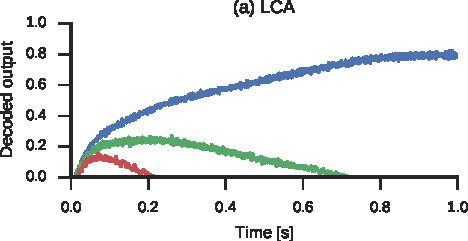
\includegraphics{figures/usher-mcclelland}
    \caption{TODO}\label{fig:usher-mcclelland}
\end{figure}

\subsection{Independent accumulator model}
The other Winner-take-all mechanism is related to the Usher-McClelland model and 
even more closely to independent accumulator models (TODO refs), but has some 
fine and important distinctions. It consists of two layers of neural 
populations. The first layer are independent accumulators obtained from 
Equation~\ref{eqn:usher-mcclelland} by setting $k = \beta = 0$ resulting in
\begin{equation}
    \begin{split}
    dx^1_i &= \lambda \rho_i \frac{dt}{\tau} \\
    x^1_i &\rightarrow \max(x^1_i, 0) \text{.}
    \end{split}
\end{equation}
The parameter $\lambda$ scales this input and is introduced because it is more 
convenient to manipulate than then the threshold parameter $\vartheta$ 
introduced below.

The second layer consists of independent non-recurrent populations that get 
input from the first layer in a one to one projection. We decode the shifted 
Heaviside function $\Theta(x^2_i - \vartheta)$ from it where $\vartheta = 0.8$ 
is a threshold value controlling how much evidence needs to be accumulated to 
produce an output. Instead of controlling this threshold, it is more convenient 
to scale the input with $\lambda$ in the context of the NEF, though 
mathematically both approaches are equivalent. As the Usher-McClelland does not 
have a threshold parameter, we do not introduce the input scaling $\lambda$ in 
that model.

The Heaviside decoded output of layer 2 projects back to layer 1 to add $x^2_i 
- 2\sum_{j \neq i} x^2_j$ to the input of $x^1_i$. As effect the choice will be 
stabilized while all other state variables will be suppressed once one of the 
accumulators reaches the threshold $\vartheta$.

TODO figure with dynamics
\begin{figure}
    \centering
    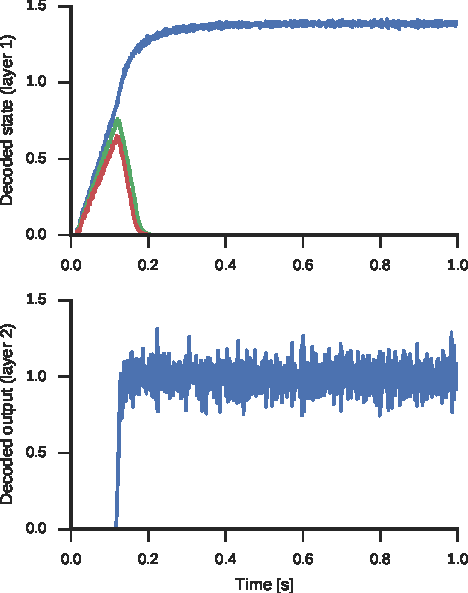
\includegraphics{figures/indacc}
    \caption{TODO}\label{fig:indacc}
\end{figure}

\section{Results}\label{sec:results}
To test and compare the two WTA mechanisms we provide an input of $\rho_i 
= u - s \delta_{1i} + \eta_i$ where $u$ is the strength of the strongest input, 
$s$ the separation to all other inputs, $\delta$ the Kronecker delta, and 
$\eta_i$ Gaussian white noise with standard deviation $\sigma$. Thus, without 
loss of generality, the first state variable receives the strongest input and 
all other state variables receive input that is $s$ less. We chose this input as 
it it represents the worse case for picking out the strongest input as $s 
\rightarrow 0$ and as one input $\rho_i \rightarrow 0$ it will have less 
influence on the overall dynamics of the two WTA mechanisms.

To evaluate the two mechanisms we use a number of metrics. First we determine 
whether the model is able to form a clear decision at all within a second of 
simulated time. To count as a clear decision at least one output needs to stay 
above 0.15 for a second after the initial second of simulation time. This 
ensures that the output is different from a 0 output which could slightly be 
above 
0 due to noise. Furthermore, we require that the largest output will be the 
  largest output for all of that second of simulation time because otherwise the 
  decision would switch.

This does not take into account whether the winning output actually corresponds 
to the strongest input, but sometimes it can be more desirable to form a clear 
decision at all than finding the actual strongest input. In other situations, 
though, the correctness of the decision might be important. So this is our next 
metric. A trial is considered correct if the model forms a clear decision and 
the largest output corresponds to the largest input.

The time it takes to form a decision can be relevant too. We define the decision 
time as how long it takes to fulfill the conditions of a clear decision.

These metrics cover the basic performance of the WTA mechanims. When using a WTA 
mechanism within larger cognitive models, the exact magnitude of the outputs can 
be important. Ideally, the output would be 1 for the winner and 0 for all other 
outputs.\footnote{Technically, the winner output could be scaled to any 
    magnitude. We use 1 here as it is most convenient to work with.} We define 
the \emph{winner error} $E_1$ as the difference of the winner output from 1 and 
the \emph{runner-up error} $E_2$ as the difference of second largest output from 
0 (negative values treated as 0). We use the average output values of the second 
  second in the simulation as the value can fluctuate over time.

These two metrics only look at the final output, but the model can produce 
transient outputs before the final decision is achieved. Within the context of 
a larger model, this can be a problem as the transient output could already be 
interpreted as a decision. Thus, we define $E_{2,\max}$ as the highest output of 
a non-winning output during the whole simulation.


We find that the ability to reach a clear decision depends on the magnitude of 
the highest input for both networks. This is not surprising. In the 
Usher-McClelland the output magnitude will be determined by the input magnitude 
of the largest input. As such the largest input needs to be above 0.2 to fulfill 
the requirements. For the independent accumulator model the input has to be 
large enough to reach the integration threshold within the time limit. By 
increasing the input scaling $\lambda$ or the time limit one could get a clear 
decision for smaller inputs within the time limit. We further find that the 
independent accumulator model is independent of the input noise and target 
separation for all tested parameters. This is not the case for the 
Usher-McClelland model as shown in Figure~TODO where the fraction of trials 
without a clear decision increases with noise and smaller target separation.
\begin{figure}
    \centering
    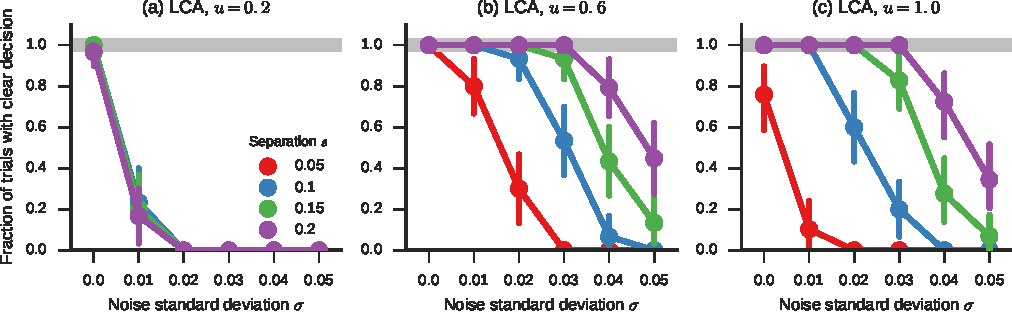
\includegraphics{figures/decisions}
    \caption{TODO}\label{fig:decisions}
\end{figure}

However, when considering the correctness of the decisions (Figure~TODO) the 
Usher-McClelland model is doing better. We can alleviate that difference to some 
degree by reducing the input scaling to $\lambda = TODO$, but perform still 
worse for small target separations when staying in the time limit.
\begin{figure*}
    \centering
    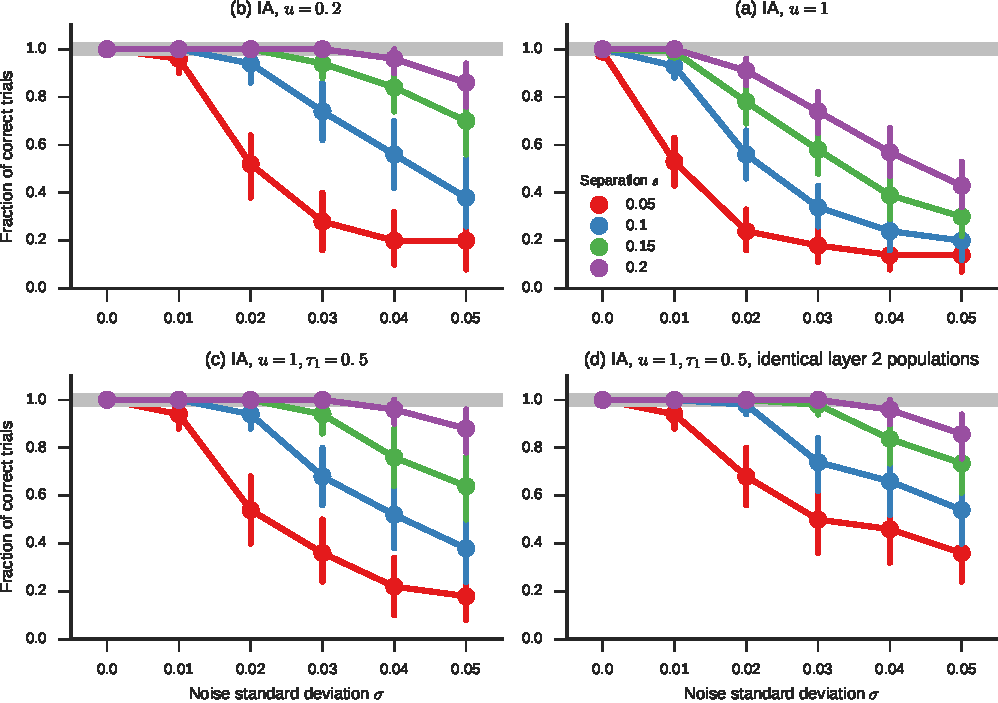
\includegraphics{figures/correct}
    \caption{TODO}\label{fig:correct}
\end{figure*}

The time required to reach a decision in the Usher-McClelland model depend 
mostly on the target separation and amount of noise on the input (Figure~TODO), 
the magnitude of the largest input is of minor influence. In contrast to that, 
in the independent accumulator model the scaled magnitude of the largest input 
is the most important factor. Depending on this magnitude the network can either 
be faster or slower than the Usher-McClelland network, but it will need more 
time to achieve the same correctness of responses. There is also a slight 
influence of target separation and input noise with an interaction of these two 
parameters (Figure~TODO).

The output of the independent accumulator model matches almost perfectly the 
specifications. This is not the case for the Usher-McClelland model 
(Figure~TODO).  For small target separations the output of the winner will stay 
below 1 and this will get worse with increased noise. As the winner output will 
try to match the largest input TODO explanation. Furthermore, the 
Usher-McClelland model will have residual outputs of non-winning choices under 
noisy conditions and with small target separations.

Finally, looking at the transient responses both models might produce outputs of 
non-winning choices. For the Usher-McClelland model these increase with noise on 
the input and, for small target separation, can approach the final output of the 
winning dimensions. For the independent accumulator model, transient output are 
smaller in noisy conditions, but can be higher than for the Usher-McClelland 
model in less noisy conditions. The magnitude of such transient responses is 
reduced by decreasing the input scaling.

\section{Discussion}\label{sec:discussion}
We do not find either one of the networks to perform better on all metrics, but 
rather they excel at slightly different things. The Usher-McClelland network is 
better suited to quickly determine the correct winner. However, under noisy 
conditions it can end up not producing a clear output at all and basically not 
making a decision at all. The independent accumulator model might not be as 
quick or find the correct winner as often, but given enough time it will 
eventually arrive at a decision and produce a clear output.

The Usher-McClelland network is especially suited for situations where 
a decision needs to be continuously adjusted. The prescribed dynamics 
essentially try to output what the currently largest input is considering some 
smoothing over time. This makes it quick to respond to changes of the input, but 
can also lead randomly switching outputs due to noise. In comparison, the 
independent accumulator model is more suited in situations where a discrete 
sequence of decisions is required. During the initial phase the model will just 
integrate evidence without any output and after making a decision, it is 
necessary to reset the model by inhibiting all layer 1 neurons. This limits the 
how quickly successive decisions can be made, but at the same time once 
a decision is made the network provides a stable output.

There are also certain considerations to be made when integrating these networks 
in larger neural or cognitive models. This integration is easy for the 
independent accumulator model as it provides a clear output. The output of the 
winning choice is also close to one which makes it easy to detect when the 
decision has been made and processing can continue. This is problematic in the 
Usher-McClelland model where we get a fluctuating output before the final 
decision and as this output can get close to the final output we cannot 
necessarily use the crossing of a threshold. Moreover, the magnitude of the 
final output depends on the magnitude of the input which is also a problem for 
using a fixed threshold.

Part of the reason why the independent accumulator model produces less correct 
responses is a systematic bias introduced in the second layer. Usually the 
neural properties are selected randomly in the NEF and this will result in 
slightly different thresholds for each of the populations before it will fire.  
It is possible to select the neural parameters in a way that all of these 
populations will have the same threshold which improves the correctness 
(Figure~TODO). However, this would require a very precise tuning of the neurons 
that might not be biologically plausible.

One critique of non-leaky accumulator models is that their ability to 
discriminate the largest input increases indefinitely with time (TODO~ref) and 
that there is no sensible stopping criterion. However, this assumes that the 
time to reach a decision has no cost. If that time has a cost, the cost of 
spending more time on the decision will at some point exceed the gain by making 
a correct decision. Furthermore, this argument assumes integration with perfect 
accuracy. But in a neural network resources are limited, as such the range and 
accuracy of values that can be represented in a neural population is limited.  
At some point this would counterbalance any additional evidence.

We did not investigate the biological plausibility here because there is 
evidence to be found for both networks (TODO references). Also, the 
implementation is spiking neurons ensures a certain level of biological 
plausibility.

TODO\@: distribution of neurons in network, looking only at cases where 
a decision could be made within the results, what about more choices, include 
a number of parameters and github url.

\section{Acknowledgments}

Place acknowledgments (including funding information) in a section at
the end of the paper.


\section{References Instructions}

Follow the APA Publication Manual for citation format, both within the
text and in the reference list, with the following exceptions: (a) do
not cite the page numbers of any book, including chapters in edited
volumes; (b) use the same format for unpublished references as for
published ones. Alphabetize references by the surnames of the authors,
with single author entries preceding multiple author entries. Order
references by the same authors by the year of publication, with the
earliest first.

Use a first level section heading, ``{\bf References}'', as shown
below. Use a hanging indent style, with the first line of the
reference flush against the left margin and subsequent lines indented
by 1/8~inch. Below are example references for a conference paper, book
chapter, journal article, dissertation, book, technical report, and
edited volume, respectively.

\bibliographystyle{apacite}

\setlength{\bibleftmargin}{.125in}
\setlength{\bibindent}{-\bibleftmargin}

\bibliography{references}


\end{document}
